% Appendix D

\chapter{Importância das Características nos Modelos de Classificação}
\label{AppendixD}

\counterwithout{table}{subsection}
\counterwithin{table}{chapter}
\counterwithout{figure}{chapter}
\counterwithin{figure}{section}
\renewcommand{\thetable}{\thechapter.\arabic{table}}
\renewcommand{\thefigure}{\thesection}

Este apêndice apresenta as figuras de importância das características dos modelos XGBoost, SVM, Regressão Logística e Random Forest nos três cenários do estudo de ablação. As figuras complementam a análise do XGBoost apresentada no Capítulo 4, permitindo comparar a forma como os diferentes modelos utilizam as características de ECG, HR/R-R e temporais. As importâncias apresentadas não devem ser comparadas diretamente entre modelos, uma vez que são calculadas através de métodos diferentes.

\section{Importância das Características no XGBoost}

\begin{sloppypar}
No XGBoost, a importância das características é obtida através de \texttt{feature\_importances\_}. Esta medida resume a contribuição de cada variável no conjunto de árvores, de acordo com o critério interno do modelo, como a frequência de utilização ou o ganho das divisões. A Tabela~\ref{tab:importance_xgboost_data} apresenta os valores dos três cenários, enquanto a Figura~\ref{fig:ablation_feature_importance_xgboost}, apresentada no Capítulo~\ref{chap:Chapter4}, ilustra a importância relativa das características.
\end{sloppypar}

\begin{table}[H]
\centering
\scriptsize
\begin{minipage}{0.32\textwidth}\centering
\textbf{Cenário A: ECG + HR/RR}
\resizebox{\linewidth}{!}{\begin{tabular}{lr}\toprule Característica & Importância \\\midrule
\texttt{HR\_min\_z} & 0,2576\\
\texttt{ECG\_energy\_z} & 0,1248\\
\texttt{cambio\_HR\_vs\_baseline\_z} & 0,0991\\
\texttt{HR\_mean\_z} & 0,0871\\
\texttt{RMSSD\_z} & 0,0701\\
\texttt{ECG\_samp\_ent\_z} & 0,0679\\
\texttt{pNN50\_z} & 0,0626\\
\texttt{HR\_max\_z} & 0,0542\\
\texttt{SDNN\_z} & 0,0392\\
\texttt{ECG\_std\_z} & 0,0381\\
\texttt{ECG\_missing\_peaks\_z} & 0,0265\\
\texttt{cambio\_RMSSD\_z} & 0,0168\\
\texttt{ECG\_mean\_z} & 0,0154\\
\texttt{HR\_mean\_ultimos\_5min\_z} & 0,0152\\
\texttt{tendencia\_HR\_z} & 0,0143\\
\texttt{ECG\_range\_z} & 0,0112\\\bottomrule\end{tabular}}
\end{minipage}\hfill
\begin{minipage}{0.32\textwidth}\centering
\textbf{Cenário B: HR/RR + temporais}
\resizebox{\linewidth}{!}{\begin{tabular}{lr}\toprule Característica & Importância \\\midrule
\texttt{HR\_min\_z} & 0,3916\\
\texttt{cambio\_HR\_vs\_baseline\_z} & 0,1847\\
\texttt{HR\_mean\_z} & 0,1552\\
\texttt{pNN50\_z} & 0,0824\\
\texttt{RMSSD\_z} & 0,0597\\
\texttt{SDNN\_z} & 0,0409\\
\texttt{HR\_max\_z} & 0,0286\\
\texttt{cambio\_RMSSD\_z} & 0,0233\\
\texttt{HR\_mean\_ultimos\_5min\_z} & 0,0196\\
\texttt{tendencia\_HR\_z} & 0,0139\\\bottomrule\end{tabular}}
\end{minipage}\hfill
\begin{minipage}{0.32\textwidth}\centering
\textbf{Cenário C: ECG}
\resizebox{\linewidth}{!}{\begin{tabular}{lr}\toprule Característica & Importância \\\midrule
\texttt{ECG\_energy\_z} & 0,2688\\
\texttt{ECG\_missing\_peaks\_z} & 0,2260\\
\texttt{ECG\_samp\_ent\_z} & 0,2080\\
\texttt{ECG\_std\_z} & 0,1176\\
\texttt{ECG\_range\_z} & 0,0899\\
\texttt{ECG\_mean\_z} & 0,0898\\\bottomrule\end{tabular}}
\end{minipage}
\caption{Importância das características no XGBoost nos três cenários.}
\label{tab:importance_xgboost_data}
\end{table}

\clearpage
\section{Importância das Características no SVM}

No SVM, especialmente quando é utilizado um kernel não linear, não existe uma propriedade equivalente a \texttt{feature\_importances\_}. Por isso, foi utilizada a importância por permutação. O procedimento compara a \textit{balanced accuracy} original com a obtida depois de permutar os valores de uma característica. Para a característica $j$, calcula-se:

\begin{equation}
I_j = S_{\mathrm{original}} - S_{\mathrm{permutada},j},
\end{equation}

onde $S$ representa a \textit{balanced accuracy}. Foram utilizadas cinco repetições por característica, com \texttt{random\_state=42}. Os valores obtidos nos três cenários são apresentados na Tabela~\ref{tab:importance_svm_data}.

\begin{table}[H]
\centering
\scriptsize
\begin{minipage}{0.32\textwidth}\centering
\textbf{Cenário A: ECG + HR/RR}
\resizebox{\linewidth}{!}{\begin{tabular}{lr}\toprule Característica & Importância \\\midrule
\texttt{ECG\_samp\_ent\_z} & 0,2523\\
\texttt{ECG\_energy\_z} & 0,2033\\
\texttt{pNN50\_z} & 0,1293\\
\texttt{HR\_mean\_z} & 0,1216\\
\texttt{cambio\_HR\_vs\_baseline\_z} & 0,1216\\
\texttt{ECG\_std\_z} & 0,1197\\
\texttt{HR\_min\_z} & 0,1031\\
\texttt{SDNN\_z} & 0,0803\\
\texttt{tendencia\_HR\_z} & 0,0726\\
\texttt{HR\_max\_z} & 0,0720\\
\texttt{ECG\_missing\_peaks\_z} & 0,0665\\
\texttt{HR\_mean\_ultimos\_5min\_z} & 0,0592\\
\texttt{RMSSD\_z} & 0,0580\\
\texttt{ECG\_range\_z} & 0,0390\\
\texttt{ECG\_mean\_z} & 0,0223\\
\texttt{cambio\_RMSSD\_z} & 0,0216\\\bottomrule\end{tabular}}
\end{minipage}\hfill
\begin{minipage}{0.32\textwidth}\centering
\textbf{Cenário B: HR/RR + temporais}
\resizebox{\linewidth}{!}{\begin{tabular}{lr}\toprule Característica & Importância \\\midrule
\texttt{pNN50\_z} & 0,0610\\
\texttt{HR\_mean\_z} & 0,0478\\
\texttt{cambio\_HR\_vs\_baseline\_z} & 0,0478\\
\texttt{HR\_min\_z} & 0,0450\\
\texttt{RMSSD\_z} & 0,0355\\
\texttt{HR\_max\_z} & 0,0270\\
\texttt{HR\_mean\_ultimos\_5min\_z} & 0,0225\\
\texttt{SDNN\_z} & 0,0198\\
\texttt{tendencia\_HR\_z} & 0,0150\\
\texttt{cambio\_RMSSD\_z} & 0,0127\\\bottomrule\end{tabular}}
\end{minipage}\hfill
\begin{minipage}{0.32\textwidth}\centering
\textbf{Cenário C: ECG}
\resizebox{\linewidth}{!}{\begin{tabular}{lr}\toprule Característica & Importância \\\midrule
\texttt{ECG\_samp\_ent\_z} & 0,2985\\
\texttt{ECG\_energy\_z} & 0,2239\\
\texttt{ECG\_std\_z} & 0,1761\\
\texttt{ECG\_missing\_peaks\_z} & 0,1423\\
\texttt{ECG\_mean\_z} & 0,1114\\
\texttt{ECG\_range\_z} & 0,0852\\\bottomrule\end{tabular}}
\end{minipage}
\caption{Importância por permutação das características no SVM nos três cenários.}
\label{tab:importance_svm_data}
\end{table}

A Figura~\ref{fig:ablation_feature_importance_svm} apresenta a importância das características no SVM, calculada através de importância por permutação. No cenário A, \texttt{ECG\_samp\_ent\_z} e \texttt{ECG\_energy\_z} apresentam os maiores valores. No cenário B, a maior importância é atribuída a \texttt{pNN50\_z}, seguida de \texttt{cambio\_HR\_vs\_baseline\_z} e \texttt{HR\_mean\_z}. No cenário C, constituído apenas por características de ECG, destacam-se \texttt{ECG\_samp\_ent\_z} e \texttt{ECG\_energy\_z}.

\begin{figure}[H]
\centering
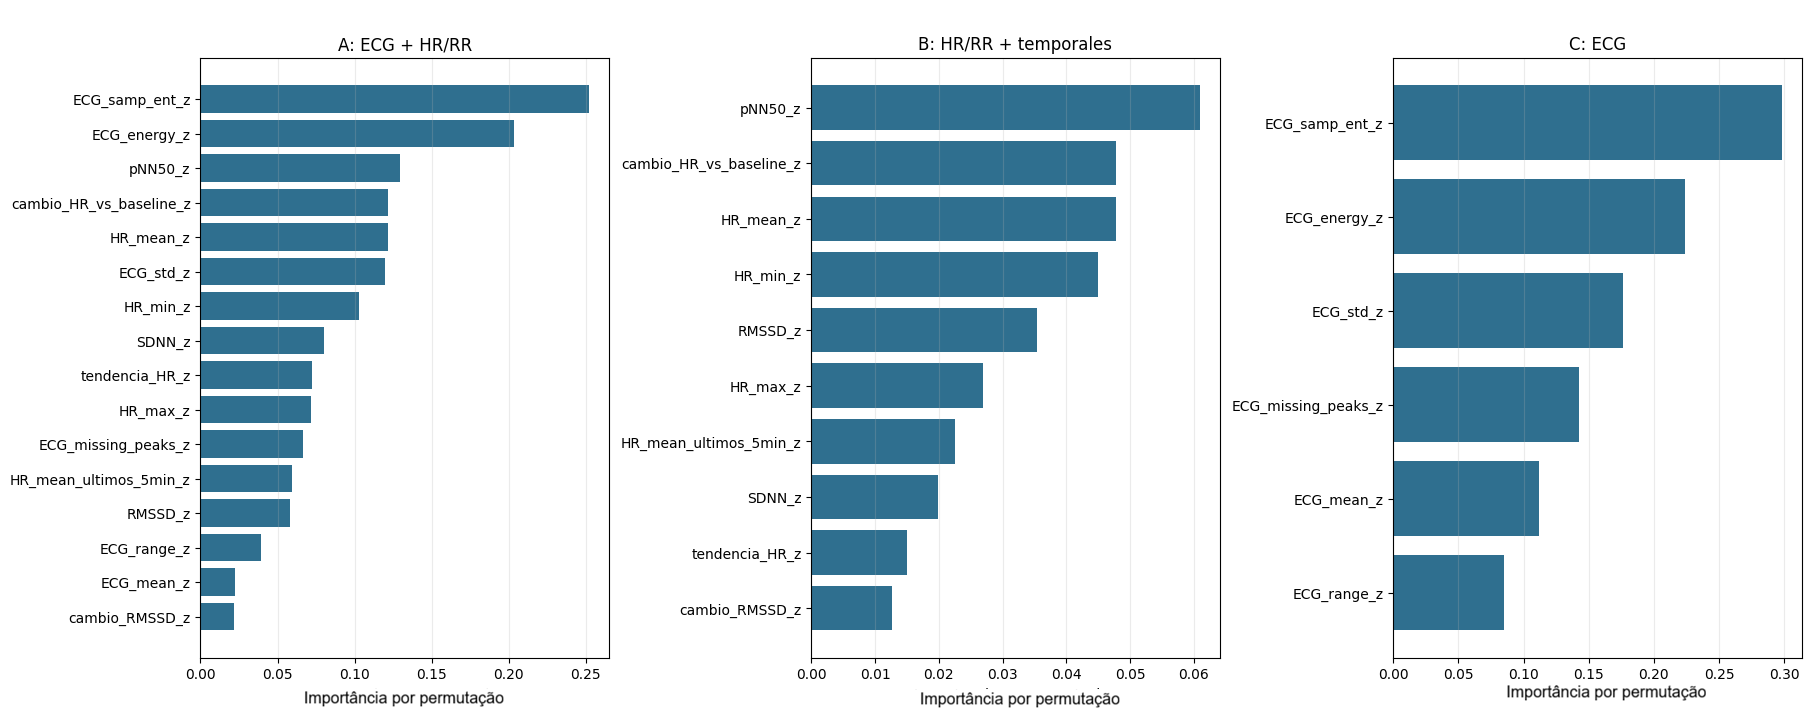
\includegraphics[width=1\textwidth]{ch4/assets/importanceSVM.png}
\caption{Importância das características por permutação no SVM nos três cenários do estudo de ablação.}
\label{fig:ablation_feature_importance_svm}
\end{figure}

\section{Importância das Características na Regressão Logística}

Na Regressão Logística, a importância de cada característica foi calculada através da média do valor absoluto dos seus coeficientes nas três classes:

\begin{equation}
I_j = \frac{1}{K}\sum_{k=1}^{K} |\beta_{k,j}|,
\end{equation}

onde $K$ é o número de classes e $\beta_{k,j}$ é o coeficiente da característica $j$ para a classe $k$. O valor absoluto mede a magnitude da influência, independentemente do seu sinal. Os valores calculados para os três cenários encontram-se na Tabela~\ref{tab:importance_logistic_data}.

\begin{table}[H]
\centering
\scriptsize
\begin{minipage}{0.32\textwidth}\centering
\textbf{Cenário A: ECG + HR/RR}
\resizebox{\linewidth}{!}{\begin{tabular}{lr}\toprule Característica & Importância \\\midrule
\texttt{ECG\_energy\_z} & 116,6476\\
\texttt{ECG\_std\_z} & 11,5302\\
\texttt{RMSSD\_z} & 3,3559\\
\texttt{ECG\_samp\_ent\_z} & 2,7714\\
\texttt{SDNN\_z} & 1,7453\\
\texttt{ECG\_mean\_z} & 1,6520\\
\texttt{ECG\_range\_z} & 1,6235\\
\texttt{ECG\_missing\_peaks\_z} & 1,2880\\
\texttt{pNN50\_z} & 1,1531\\
\texttt{cambio\_RMSSD\_z} & 1,0886\\
\texttt{HR\_max\_z} & 0,8627\\
\texttt{HR\_min\_z} & 0,5526\\
\texttt{cambio\_HR\_vs\_baseline\_z} & 0,5490\\
\texttt{HR\_mean\_z} & 0,5490\\
\texttt{tendencia\_HR\_z} & 0,1431\\
\texttt{HR\_mean\_ultimos\_5min\_z} & 0,0796\\\bottomrule\end{tabular}}
\end{minipage}\hfill
\begin{minipage}{0.32\textwidth}\centering
\textbf{Cenário B: HR/RR + temporais}
\resizebox{\linewidth}{!}{\begin{tabular}{lr}\toprule Característica & Importância \\\midrule
\texttt{HR\_min\_z} & 0,9839\\
\texttt{RMSSD\_z} & 0,6872\\
\texttt{pNN50\_z} & 0,5506\\
\texttt{cambio\_HR\_vs\_baseline\_z} & 0,3099\\
\texttt{HR\_mean\_z} & 0,3099\\
\texttt{HR\_mean\_ultimos\_5min\_z} & 0,2558\\
\texttt{cambio\_RMSSD\_z} & 0,2480\\
\texttt{SDNN\_z} & 0,1190\\
\texttt{HR\_max\_z} & 0,1183\\
\texttt{tendencia\_HR\_z} & 0,0611\\\bottomrule\end{tabular}}
\end{minipage}\hfill
\begin{minipage}{0.32\textwidth}\centering
\textbf{Cenário C: ECG}
\resizebox{\linewidth}{!}{\begin{tabular}{lr}\toprule Característica & Importância \\\midrule
\texttt{ECG\_energy\_z} & 44,8192\\
\texttt{ECG\_std\_z} & 5,2296\\
\texttt{ECG\_range\_z} & 1,8034\\
\texttt{ECG\_samp\_ent\_z} & 1,4279\\
\texttt{ECG\_mean\_z} & 1,2172\\
\texttt{ECG\_missing\_peaks\_z} & 0,1657\\\bottomrule\end{tabular}}
\end{minipage}
\caption{Importância média absoluta dos coeficientes da Regressão Logística nos três cenários.}
\label{tab:importance_logistic_data}
\end{table}

A Figura~\ref{fig:ablation_feature_importance_logistic} apresenta os coeficientes médios em valor absoluto da Regressão Logística nos três cenários. No cenário A, \texttt{ECG\_energy\_z} apresenta uma importância claramente superior às restantes características. No cenário B, as maiores contribuições correspondem a \texttt{HR\_min\_z}, \texttt{RMSSD\_z} e \texttt{pNN50\_z}. No cenário C, \texttt{ECG\_energy\_z} volta a destacar-se, enquanto as restantes características de ECG apresentam contribuições bastante inferiores.

\begin{figure}[H]
\centering
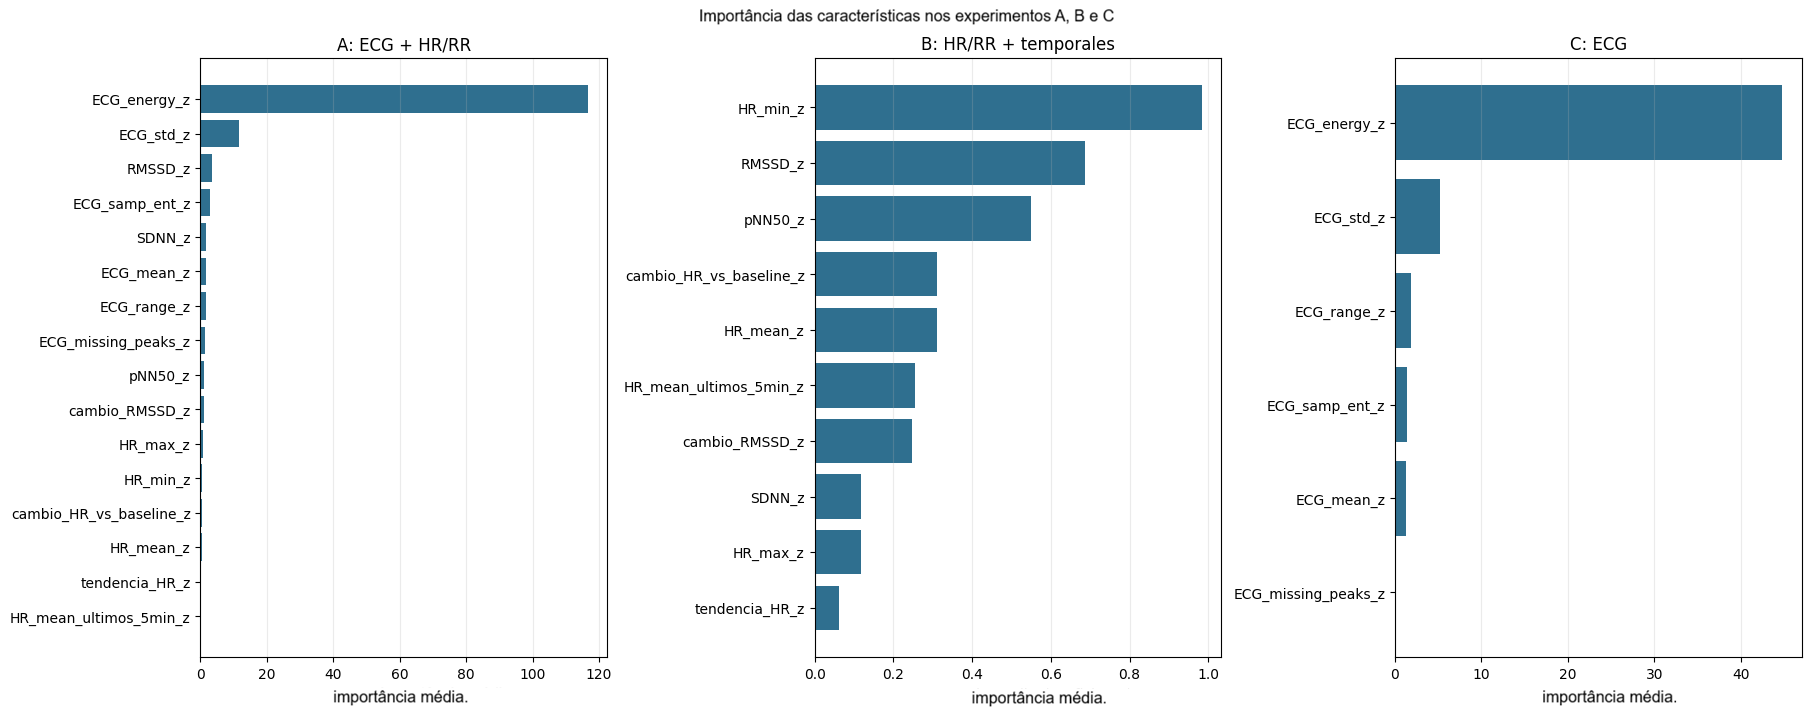
\includegraphics[width=1\textwidth]{ch4/assets/importanceLOGISTIC.png}
\caption{Importância média das características, em valor absoluto dos coeficientes, na Regressão Logística nos três cenários do estudo de ablação.}
\label{fig:ablation_feature_importance_logistic}
\end{figure}

\section{Importância das Características no Random Forest}

No Random Forest, utiliza-se diretamente \texttt{feature\_importances\_}. Esta medida corresponde à redução média de impureza produzida por cada característica nas árvores do bosque. Embora seja útil para descrever a forma como o modelo utiliza as variáveis, pode ser influenciada por características contínuas, por muitos pontos de separação e por variáveis correlacionadas, não constituindo uma relação causal. Os valores obtidos nos três cenários são apresentados na Tabela~\ref{tab:importance_random_data}.

\begin{table}[H]
\centering
\scriptsize
\begin{minipage}{0.32\textwidth}\centering
\textbf{Cenário A: ECG + HR/RR}
\resizebox{\linewidth}{!}{\begin{tabular}{lr}\toprule Característica & Importância \\\midrule
\texttt{ECG\_energy\_z} & 0,2006\\
\texttt{ECG\_samp\_ent\_z} & 0,1937\\
\texttt{ECG\_std\_z} & 0,1197\\
\texttt{HR\_min\_z} & 0,0834\\
\texttt{cambio\_HR\_vs\_baseline\_z} & 0,0675\\
\texttt{HR\_mean\_z} & 0,0629\\
\texttt{ECG\_range\_z} & 0,0522\\
\texttt{RMSSD\_z} & 0,0478\\
\texttt{pNN50\_z} & 0,0429\\
\texttt{ECG\_mean\_z} & 0,0410\\
\texttt{SDNN\_z} & 0,0308\\
\texttt{HR\_mean\_ultimos\_5min\_z} & 0,0186\\
\texttt{HR\_max\_z} & 0,0126\\
\texttt{ECG\_missing\_peaks\_z} & 0,0099\\
\texttt{cambio\_RMSSD\_z} & 0,0094\\
\texttt{tendencia\_HR\_z} & 0,0069\\\bottomrule\end{tabular}}
\end{minipage}\hfill
\begin{minipage}{0.32\textwidth}\centering
\textbf{Cenário B: HR/RR + temporais}
\resizebox{\linewidth}{!}{\begin{tabular}{lr}\toprule Característica & Importância \\\midrule
\texttt{HR\_min\_z} & 0,2269\\
\texttt{HR\_mean\_z} & 0,1918\\
\texttt{cambio\_HR\_vs\_baseline\_z} & 0,1854\\
\texttt{pNN50\_z} & 0,1188\\
\texttt{RMSSD\_z} & 0,1140\\
\texttt{SDNN\_z} & 0,0575\\
\texttt{HR\_mean\_ultimos\_5min\_z} & 0,0517\\
\texttt{HR\_max\_z} & 0,0246\\
\texttt{cambio\_RMSSD\_z} & 0,0184\\
\texttt{tendencia\_HR\_z} & 0,0109\\\bottomrule\end{tabular}}
\end{minipage}\hfill
\begin{minipage}{0.32\textwidth}\centering
\textbf{Cenário C: ECG}
\resizebox{\linewidth}{!}{\begin{tabular}{lr}\toprule Característica & Importância \\\midrule
\texttt{ECG\_samp\_ent\_z} & 0,2485\\
\texttt{ECG\_energy\_z} & 0,2352\\
\texttt{ECG\_missing\_peaks\_z} & 0,1664\\
\texttt{ECG\_std\_z} & 0,1441\\
\texttt{ECG\_mean\_z} & 0,1040\\
\texttt{ECG\_range\_z} & 0,1017\\\bottomrule\end{tabular}}
\end{minipage}
\caption{Importância das características no Random Forest nos três cenários.}
\label{tab:importance_random_data}
\end{table}

A Figura~\ref{fig:ablation_feature_importance_random} apresenta a importância das características no Random Forest. No cenário A, \texttt{ECG\_energy\_z} e \texttt{ECG\_samp\_ent\_z} são as características mais relevantes. No cenário B, a importância concentra-se em \texttt{HR\_min\_z}, \texttt{HR\_mean\_z} e \texttt{cambio\_HR\_vs\_baseline\_z}. No cenário C, as características mais relevantes são \texttt{ECG\_samp\_ent\_z}, \texttt{ECG\_energy\_z} e \texttt{ECG\_missing\_peaks\_z}. Estes resultados confirmam que a importância relativa das variáveis depende do conjunto de características disponível em cada cenário.

\begin{figure}[H]
\centering
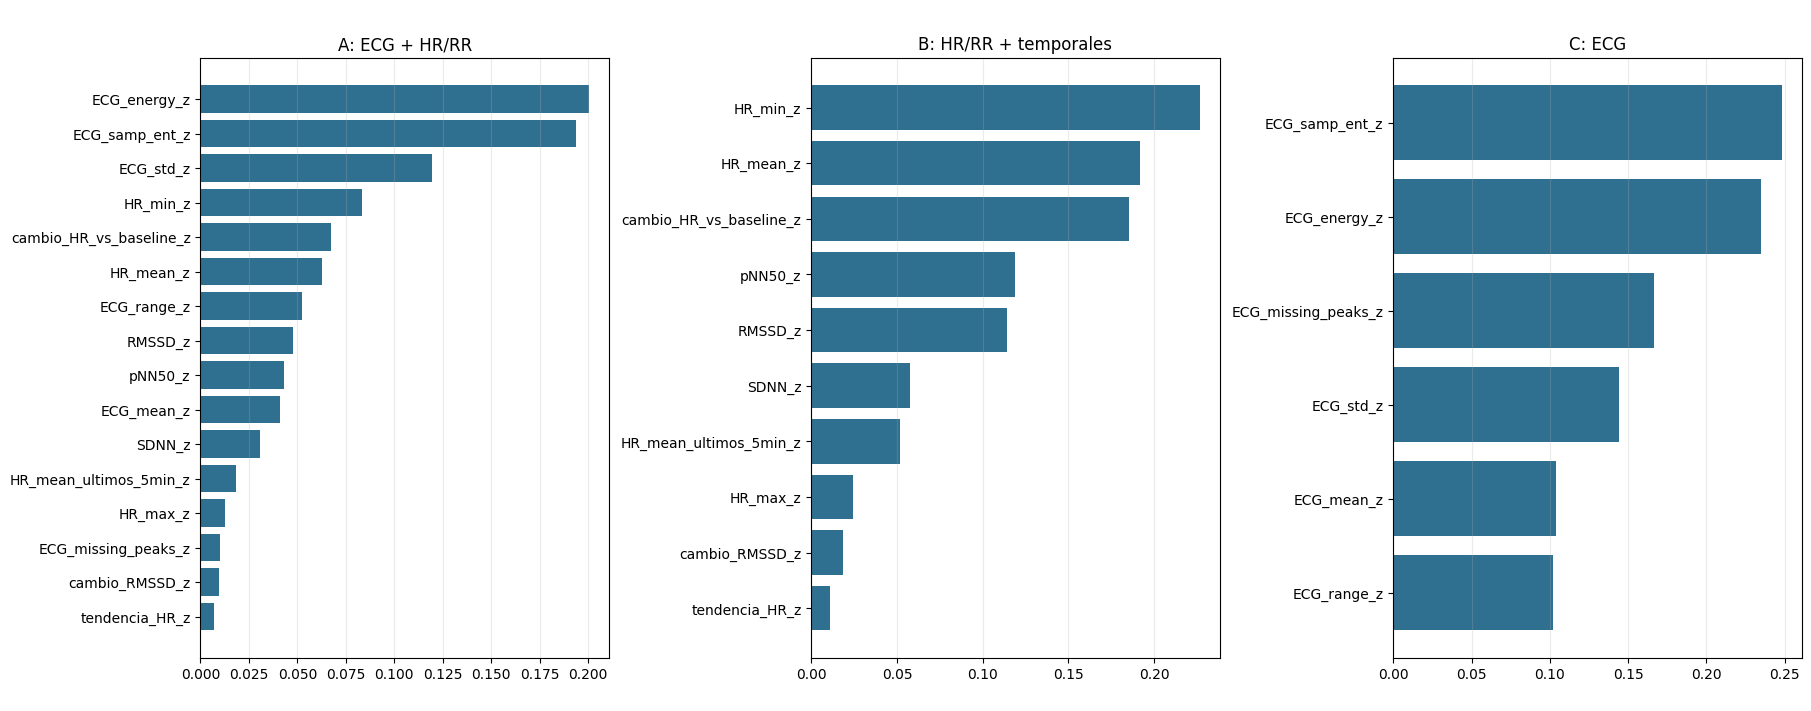
\includegraphics[width=1\textwidth]{ch4/assets/importanceRANDOM.png}
\caption{Importância relativa das características no Random Forest nos três cenários do estudo de ablação.}
\label{fig:ablation_feature_importance_random}
\end{figure}
